\appendix

\section{Hilfreiches}

\subsection{Inverse in Galois-Feldern}

\textbf{Additive Inverse}

gegeben: $-3$ in $GF(5)$

gesucht: additive Inverse

bedeutet: $3 + x \mod 5 = n = 0$

$n$: neutrales Element der Addition ($=0$)

$x = 2$ , da $3 + 2 = 5$ und $5 \mod 5 = 0$

daher: $-3 = 2$

\underline{oder}: mit Tabelle

gegebene Zahl als Index behandeln, passenden Wert raussuchen

\begin{tabular}{ c | c | c | c | c | c | c | c | c | c | c | c | }
    Index & -3 & -2 & -1 & 0 & 1 & 2 & 3 & 4 & 5 & 6\\
    \hline
    Wert  & 2  &  3 &  4  & 0 & 1 & 2 & 3 & 4 & 0 & 1
\end{tabular}

\textbf{Multiplikative/modulare Inverse}

gegeben: $2^{-1}$ in $GF(7)$

gesucht: multiplikative Inverse

bedeutet: $2^{1} \cdot x \mod 7 = n = 1$

$n$: neutrales Element der Multiplikation ($=1$)

$x = 4$ , da $2^{1} \cdot 4 = 8$ und $8 \mod 7 = 1$

daher: $2^{-1} = 4$

\underline{oder}: mit Logarithmentafel

gegebene Potenz als Index behandeln, passenden Wert raussuchen

\begin{tabular}{ c | c | c | c | c | c | c | c | c | c | c | c | }
    Index  & -3 & -2 & -1 & 0 & 1 & 2 & 3 & 4 & 5 & 6\\
    \hline
    Wert   &  1 &  2 &  4 & 1 & 2 & 4 & 1 & 2 & 4 & 1
\end{tabular}

\subsection{Rechnen im Erweiterungskörper}

Bsp.: $GF(2^4)$ mit $p(x) = x^4 + x + 1$

\textbf{Addition}
%// TODO

\textbf{Multiplikation}
%// TODO

gegeben $5 \cdot 6 = (\alpha^2 + 1) \cdot (\alpha^2 + \alpha)$

\subsection{Syndromstellen aus Generatorpolynom}

Bsp.: $GF(5)$ mit $\alpha = 2$

gegeben $g(x) = x^2 + 5x + 4$

$\hookrightarrow$ 2 Syndromstellen

Suchen über stures Einsetzen der Elemente des $GF(5)$:

$g(\alpha^{-0}) = \alpha^{-0^2} + 3\alpha^{-0} + 2 = 1 + 3 + 2 = 1$

$\hookrightarrow$ Position 0 keine Syndromstelle 

$g(\alpha^{-1}) = \alpha^{-1^2} + 3 \alpha^{-1} + 2 = 3^2 + 3 \cdot 3 + 2 = 0$

$\hookrightarrow$ Position 1 ist Syndromstelle

$g(\alpha^{-2}) = \alpha^{-2^2} + 3 \cdot \alpha^{-2} + 2 = 4^2 + 3 \cdot 3^2 + 2 = 0$

$\hookrightarrow$ Position 2 ist Syndromstelle

\subsection{ABC/PQ-Formel}

\textbf{ABC:} $ax^2 + bx + c = 0$

$\displaystyle{
    x_{1,2} = \frac{-b \pm \sqrt{ b^2 - 4ac }}{2a}
}$

\textbf{PQ:} $x^2 + px + q$

$\displaystyle{
    x_{1,2} = -\frac{p}{2} \pm \sqrt{\left(\frac{p}{2}\right)^2 - q}
}$

\section{Polynome}

\subsection{Polynommultiplikation}

\subsection{Polynomdivision}

\textbf{allgemein:}

gegeben: $(6x^3-2x^2+x+3) : (x^2-x+1)$

\polylongdiv[style=D]{6x^3-2x^2+x+3}{x^2-x+1}

Quotient $q(x) = 6x + 4$

Rest $r(x) = - x - 1$

\textbf{Horner-Schema}

zur Polynomdivision mit Linearfaktor

Rest der Division mit $(x - x_0)$ ist Wert des Polynoms an der Stelle $x_0$

gegeben: $p(x) = 3x^3 + 2x^2 - 5x - 10$

$\begin{array}{c|cccc|c}
    & x^3 & x^2 & x^1 & x^0 & 2\\
    & 3   & 2   & -5  & -10 & \\
    &     & 6   & 16  & 22  \\ \hline
    & 3   & 8   & 11  & \multicolumn{1}{c|}{12}   &
\end{array}$

Quotient: $q(x) = 3x^2 + 8x + 11$

Rest: $r(x) = 12 = p(2)$

\section{Lineare Algebra}

\textbf{Matrix-Multiplikation}

$\displaystyle{
    A \cdot B = 
    \begin{pmatrix}
        a & b\\
        c & d\\
        e & f
    \end{pmatrix}_{\color{red} 3 , \color{green} 2 }
    \begin{pmatrix}
        g & h\\
        i & j
    \end{pmatrix}_{\color{green} 2, \color{blue} 2}
    = 
    \begin{pmatrix}
        a g + b i & a h + b j\\
        c g + d i & c h + d j\\
        e g + f i & e h + f j
    \end{pmatrix}_{\color{red} 3, \color{blue} 2}
}$

$\displaystyle{
    \vec{v} \cdot \vec{w}^T = 
    \begin{pmatrix}
        a \\
        b\\
        c
    \end{pmatrix}
    \cdot
    \begin{pmatrix}
        d & e & f
    \end{pmatrix}
    = 
    \begin{pmatrix}
        a \cdot d & a \cdot e & a \cdot f\\
        b \cdot d & b \cdot e & b \cdot f\\
        c \cdot d & c \cdot e & c \cdot f
    \end{pmatrix}
}$

Skalarprodukt:

$\displaystyle{
    \vec{v}^T \cdot \vec{w} = 
    \begin{pmatrix}
        a & b & c
    \end{pmatrix}
    \cdot
    \begin{pmatrix}
        d\\
        e\\
        f
    \end{pmatrix}
    = a \cdot d + b \cdot e + c \cdot f
}$

bei komplexen Vektoren:
$\displaystyle{
    \vec{v}^H \cdot \vec{w}
}$

\textbf{Transponieren}

Zeilen werden Spalten, Spalten werden Zeilen

$\displaystyle{
    A^T =
    \begin{pmatrix}
        a & b & c\\
        d & e & f
    \end{pmatrix}^T
    =
    \begin{pmatrix}
        a & d\\
        b & e\\
        c & f
    \end{pmatrix}
}$

\textbf{Invertieren}

für 2x2-Matrizen:

$\displaystyle{
    A^{-1} =
    \begin{pmatrix}
        a & b\\
        c & d
    \end{pmatrix}^{-1}
    = \frac{1}{ad - bc}
    \begin{pmatrix}
        d & -c\\
        -b & a
    \end{pmatrix}
}$

\textbf{Diagonale Matrix}

$\displaystyle{
    \begin{pmatrix}
        1 & 0 & 0\\
        0 & -5 & 0\\
        0 & 0 & 3
    \end{pmatrix}
}$

Spalten der Matrix sind Eigenvektoren

1; -5; 3 sind die Eigenwerte der Eigenvektoren

\textbf{Hermitesche Matrix}

nur für quadratische Matrizen

$\displaystyle{
    A = A^H = (A^*)^T =
    \begin{pmatrix}
        1 & 5 - j & 3j\\
        5 + j & 2 & 3 - 2j\\
        -3j & 3 + 2j & 3 +4j
    \end{pmatrix}
}$

Eigenvektoren von hermiteschen Matrizen sind orthogonal

\textbf{Unitäre Matrix}

$\displaystyle{
    A \cdot A^H = k \cdot I
}$

$k$: Skalierungsfaktor (bei skaliert unitären Matrizen)

\textbf{Toeplitz-Struktur}

Eine Matrix hat Toeplitz-Struktur, wenn alle Diagonalen parallel zur Hauptdiagonalen, die gleichen Elemente enthalten:

$\displaystyle{
    T =
    \begin{pmatrix}
        0 & -2 & -5 & -3\\
        1 & 0 & -2 & -5 \\
        2 & 1 & 0 & -2  \\
        3 & 2 & 1 & 0
    \end{pmatrix}
}$
 
Hermitesche Toeplitz-Matrizen sind positiv oder negativ definit, abhängig vom Vorzeichen der
Elemente auf der Hauptdiagonalen

\textbf{Vandermonde-Matrix}

Spalten: Indezes gleich\\
Zeilen: Potenzen gleich

$\displaystyle{
    S =
    \begin{pmatrix}
        1 & 1 & ... & 1\\
        x_0^1 & x_1^1 & ... & x_{N-1}^1\\
        x_0^2 & x_1^2 & ... & x_{N-1}^2\\
        ... & ... & ... & ...\\
        x_0^{N-1} & x_1^{N-1} & ... & x_{N-1}^{N-1}
    \end{pmatrix}
}$

\textbf{Determinante}

nur für quadratische Matrizen

für $2 \times 2$-Matrix:

$\displaystyle{
    det(A) = det\left[
        \begin{pmatrix}
            a & b\\
            c & d
        \end{pmatrix}
    \right] = 
    a \cdot d - b\cdot c
}$

für $3 \times 3$-Matrix:

$\displaystyle{
    det(C) = det\left[
        \begin{pmatrix}
            a & b & c\\
            d & e & f\\
            g & h & i
        \end{pmatrix}
    \right]
}$

$\displaystyle{
    = a \cdot det\left[ \begin{pmatrix}
        e & f\\
        h & i
        \end{pmatrix} \right]
    - b \cdot det\left[ \begin{pmatrix}
        d & f\\
        g & i
        \end{pmatrix} \right]
    + c \cdot det\left[ \begin{pmatrix}
        d & e\\
        g & h
        \end{pmatrix} \right]
}$

\textbf{Rang einer Matrix}

Eine Matrix hat vollen Rang, wenn die Determinante ungleich 0 ist

Ist die Determinante gleich 0, ist die Matrix/das Gleichungssystem überbestimmt

\textbf{Eigenvektoren/ Eigenwerte}

Eigenvektoren einer Matrix werden bei einer Matrixtransformation nur in ihrer Länge geändert,
nicht in ihrer Richtung

Faktor, um den ein Eigenvektor gedehnt oder gestaucht wird, ist der zum Eigenvektor zugehöriger
Eigenwert $\lambda$

$\displaystyle{
    A \vec{v} = \lambda \vec{v}
}$

$\displaystyle{
    (A - \lambda I) \vec{v} = \vec{0}
}$

$A$: Matrix\\
$\vec{v}$: Eigenvektor\\
$\lambda$: Eigenwert(e)\\
$I$: Einheitsmatrix

Eigenwerte von positiv (oder negativ) definiten Matrix sind immer positiv (oder negativ)


\section{Digitale Signalverarbeitung}

\textbf{Diskretisierung und Fensterung}

Diskretisierung \laplace \; Periodische Fortsetzung\\
Diskretisierung \Laplace \; Periodische Fortsetzung\\
Begrenzung $\rightarrow$ Leck-Effekt

\textbf{Fourier-Transformation (kontinuierlich)}

$\displaystyle{
    X(f) = \int_{-\infty}^{\infty} x(t) \cdot e^{-j2\pi ft} \, dt
}$

\textbf{DFT}

$\displaystyle{
    X(n) = \sum_{k=0}^{N-1} x(k) \cdot e^{-j2\pi \frac{nk}{N}}
}$

$n$: Frequenzindex\\
$k$: Zeitindex

\textbf{Auflösung DFT}

$\displaystyle{
    \Delta f = \frac{f_a}{N} = \frac{1}{t_a \cdot N} = \frac{1}{\Delta t}
}$

$\Delta f$: spektrale Auflösung\\
$f_a$: Abtastfrequenz\\
$t_a$: Abtastrate\\
$N$: Anzahl Abtastwerte\\
$\Delta t$: Messdauer

\textbf{Fensterung}

Fensterung im Zeitbereich $\rightarrow$ Multiplikation mit Fensterfunktion \laplace \; Faltung mit zur Fensterfunktion zugehörigem Spektrum

\textbf{Dirichlet-Kern}

abgetastete Rechteckfunktion \laplace \; Dirichlet-Kern

Definition der Dirichlet-Kerns der Länge $N+1$:

$\displaystyle{
    D(x) = \sum_{n=-\frac{N}{2}}^{\frac{N}{2}} e^{jnx} =
    \frac{\sin\left( \left( \frac{N + 1}{2} \right) x \right)}{\sin\left( \frac{x}{2} \right)}
}$

$x = 2\pi fT_a$

Bsp: 11:

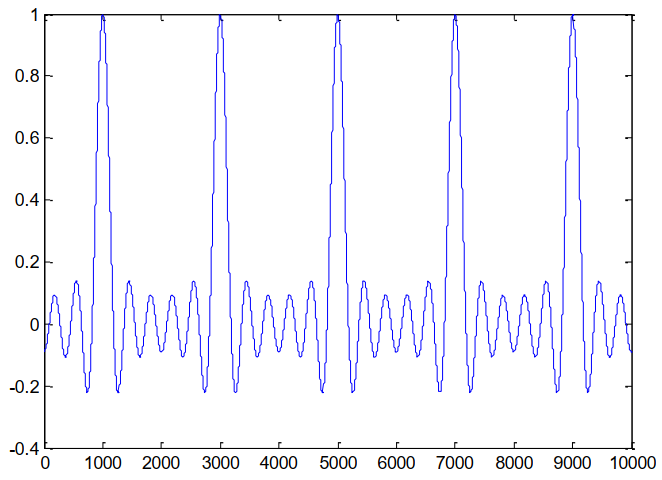
\includegraphics[width=6cm]{img/dirichlet-kern.png}

Eigenschaften:

Hauptwert hat Höhe $N+1$\\
Nullstellen, bei $\displaystyle{
    f = \frac{f_a}{N+1} \cdot k
}$ für
$\displaystyle{
    k \in \mathbf{N}
}$\\
Hauptwert periodisch mit $f_a$

\textbf{z-Transformation}

$\displaystyle{
    z = e^{j2\pi \frac{f}{f_a}}
}$

$\displaystyle{
    H(f) = H(z) \bigg \vert _{z=e^{j2\pi \frac{f}{f_a}}}
}$

\textbf{Reiner FIR-Filter}

kanonische Form

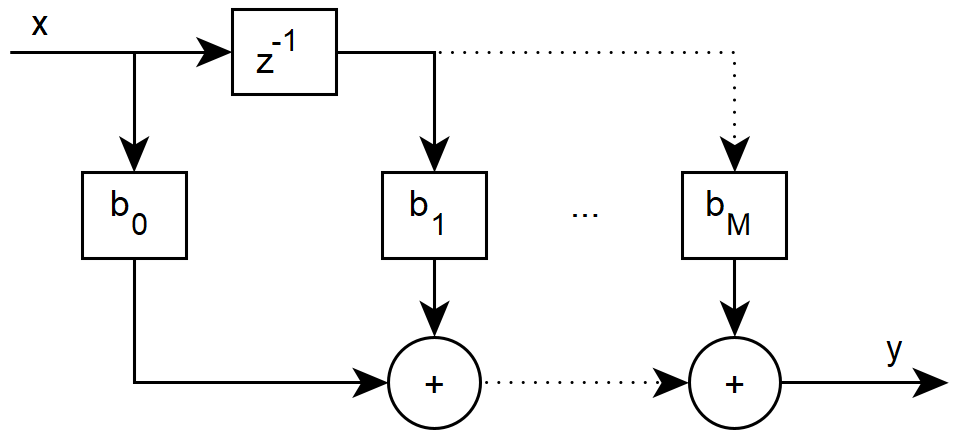
\includegraphics[width=6cm]{img/fir.png}

$\displaystyle{
    H(z) = \frac{Y(z)}{X(z)} = b_0 + b_1 \cdot z^{-1} + ... + b_M \cdot z^{-M}
}$

$\displaystyle{
    y(t) = b_0 \cdot x(t) + b_1 \cdot x(t-1) + ... + b_M \cdot x(t-M)
}$

\textbf{Reiner IIR-Filter}

kanonische Form

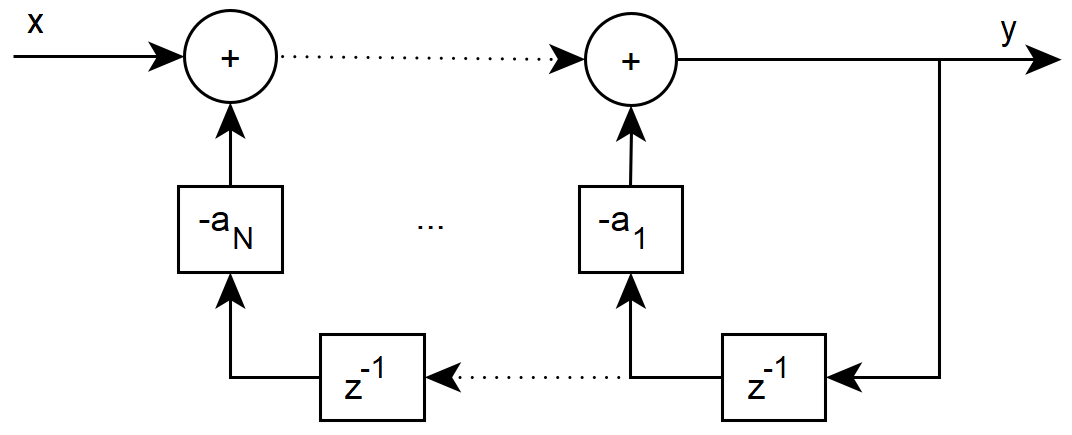
\includegraphics[width=6.5cm]{img/iir.png}

$\displaystyle{
    H(z) = \frac{1}{1 + a_1 \cdot z^{-1} + ... + a_N \cdot z^{-N}}
}$

$\displaystyle{
    y(t) = x(t) - a_1 \cdot y(t-1) - ... - a_n \cdot y(t-N)
}$

\section{Wahrscheinlichkeitstheorie}

\subsection{Satz von Bayes}

$\displaystyle{
    P(A|B) \cdot P(B) = P(B|A) \cdot P(A) = P(A,B)
}$

$\displaystyle{
    P(A|B) = \frac{P(B|A)}{P(B)} \cdot P(A)
}$

\subsection{Kombinatorik}

\subsubsection{Permutation}

\textbf{Ohne Wiederholung}

Anordung \underline{aller} möglicher, unterscheidbarer Ereignisse, kein Ereignisse tritt doppelt auf

$\displaystyle{
    M = N!
}$

\textbf{Beispiel}: In einem Glas sind 5 verschiedenfarbige Bonbons. Wie viele Möglichkeiten gibt es,
alle aus dem Glas zu nehmen? (ohne Zurücklegen)

$\hookrightarrow M = N! = 5! = 120$

\textbf{Mit Wiederholung}

Anordung aller möglicher Ereignisse, von welchen manche nicht unterscheidbar sind

$\displaystyle{
    M = \frac{N!}{K_1! \cdot ... \cdot K_s!}
}$

$K_x$: Gibt an, wie viele ununterscheidbare Ereignisse es pro Ereignis gibt

\textbf{Beispiel}: In einem Glas liegen 2 blaue, 2 rote und ein grünes Bonbon. Wie viele Möglichkeiten gibt es
alle aus dem Glas zu nehmen? (Ohne Zurücklegen)

$\displaystyle{
    \hookrightarrow \frac{5!}{2! \cdot 2! \cdot 1!} = 30
}$

$N$: Anzahl der möglichen Ereignisse\\
$M$: Anzahl der Permutationen

\subsubsection{Variation}

\textbf{Ohne Wiederholung}

Zusammenstellung von $K$ Ereignissen; Reihenfolge relevant

$\displaystyle{
    M = \frac{N!}{(N - K)!}
}$

\textbf{Beispiel}: In einem Glas liegen 5 verschiedenfarbige Bonbons. Wie viele Möglichkeiten gibt es, 3
Bonbons herauszunehmen? (Ohne Zurücklegen)

$\displaystyle{
    \hookrightarrow M = \frac{5!}{(5-2)!} = \frac{5!}{2!} = 60
}$

\textbf{Mit Wiederholung}

$\displaystyle{
    M = N^{K}
}$

\textbf{Beispiel}: In einem Glas liegen 5 verschiedenfarbige Bonbons. Wie viele Möglichkeiten gibt es, 3
Bonbons herauszunehmen? (Mit Zurücklegen)

$\displaystyle{
    \hookrightarrow M = 5^3 = 125
}$

$M$: Anzahl der Variationen\\
$N$: Anzahl der möglichen Ereignisse\\
$K$: Anzahl der zusammengestellten Ereignisse (Ordnung)

\subsubsection{Kombination}

Wie Variation, Reihenfolge aber irrelevant (vgl. Lottoziehung)

\textbf{Ohne Wiederholung}

$\displaystyle{
    M = \begin{pmatrix}
        N\\
        K
    \end{pmatrix}
    = \frac{N!}{K! \cdot (N - K)!}
}$

\textbf{Mit Wiederholung}

$\displaystyle{
    M = \begin{pmatrix}
        N + K - 1\\
        K
    \end{pmatrix} 
    = \frac{(N + K - 1)!}{K! \cdot (N - 1)!}
}$

$M$: Anzahl der Kombinationen\\
$N$: Anzahl der möglichen Ereignisse\\
$K$: Anzahl der zusammengestellten Ereignisse (Ordnung)